\documentclass{gretsi}

\usepackage[utf8]{inputenc}
\usepackage[T1]{fontenc}
\usepackage{amsmath, amssymb}
\usepackage[english,french]{babel}
  \usepackage{times}	
\usepackage{algorithm}
\usepackage[noend]{algpseudocode}
\usepackage{color}
\usepackage{graphicx}
\usepackage[font=scriptsize]{caption}
%\usepackage{enumitem}

%Gummi|065|=)
\title{Groupement automatique pour l'analyse du spectre singulier}

\auteur{\coord{Thomas}{Moreau}{1, 2},
        \coord{Laurent}{Oudre}{3, 2},
    \coord{Nicolas}{Vayatis}{1, 2}}

\adresse{\affil{1}{CMLA - ENS Cachan - 64 Avenue du Président Wilson, 94230 Cachan}
         \affil{2}{COGNAC-G - Université Paris Descartes - 45, rue des Saints-Pères, 75006 Paris}
         \affil{3}{L2TI - Université Paris 13 - 99 Avenue Jean Baptiste Clément, 93430 Villetaneuse}}
         
\email{\footnotesize thomas.moreau@cmla.ens-cachan.fr, laurent.oudre@univ-paris13.fr, nicolas.vayatis@cmla.ens-cachan.fr}

\makeatletter
\def\BState{\State\hskip-\ALG@thistlm}
\makeatother
\def\HH{\mathcal H}

\resumefrancais{Cet article introduit différentes stratégies de groupement automatique pour les composantes issues d'une analyse du spectre singulier (SSA). Cette étape, cruciale à la reconstruction de composantes haut niveau, permet de séparer les différentes dynamiques présentes dans un signal. Plusieurs stratégies  sont comparées dans un cadre d'évaluation unifié afin de mettre en lumière les spécificités de chacune.}
\resumeanglais{This paper introduce several automatic grouping strategies for Singular Spectrum Analysis (SSA) components. This step is useful to retrieve meaningful insight about the temporal dynamics of the series. An unifying framework is proposed to evaluate and compare the efficiency of different methods.}


\newcommand{\R}{\mathbb R}
\newcommand{\serie}[1]{(#1_i)_{1 \le i\le T}}
\newcommand{\val}[3]{(#1_1 #3 \dots #3 #1_#2)}
\newcommand{\vect}[3]{(#1_1 #3 \dots #3 #1_#2)}
\newcommand{\set}[1]{\left \{ 1, \dots, #1 \right \}}
\newcommand{\inter}{\left[0, 1\right]}


\begin{document}

\maketitle


\section{Introduction}
\label{sec:intro}

\begin{sloppypar}
L'analyse du spectre singulier (en anglais SSA : Singular Spectral Analysis) est une technique introduite par Vautard et al \cite{vautard_89_SSA} permettant d'obtenir de manière simple une décomposition du signal en composantes de tendance, de saisonnalité (harmoniques) et de bruit.
Elle est principalement utilisée en finance ou en météorologie où les séries étudiées sont souvent courtes et bruitées.
De nombreuses publications ont montré la pertinence de la SSA dans ces contextes, où cette décomposition permet d'apporter de l'information sur les mécanismes produisant ces séries mais aussi de formuler des modèles de prédiction.
%Cette approche peut aussi s'interpréter comme une technique de décomposition en dictionnaires empiriques.
%Les propriétés particulières de chaque élément dudicitonnaire peuvent données d'intéressantes informations sur la série de base.
Néanmoins, cette technique a été rarement utilisée sur d'autres signaux, principalement à cause de son manque d'automatisation.
La pertinence des décompositions obtenues dépend en effet énormément du regroupement des composantes extraites, et résoudre cette tâche de façon manuelle peut s'avérer laborieux.
Dans cet article, nous proposons un cadre permettant l'évaluation et la comparaison de différentes stratégies de regroupement automatique (existantes et originales).
%Cet article a pour but de présenter différentes stratégies de regroupement automatique (existantes et originales) ainsi qu'un cadre permettant leur évaluation et leur comparaison.
\end{sloppypar}

\noindent\textbf{Rappels sur la SSA.}\label{sub:rap}
On considère un signal fini échantillonné $x = \val{x}{T}{,}$ et un entier $K \in \left \{ 1, \dots, T/2 \right \}$.
La matrice de K-trajectoire $X^{(K)} \in \R^{K\times L}$ de la série $x$ est défini par:
\begin{sloppypar}
\begin{equation} 
    X^{(K)} =
    \begin{bmatrix}
	    x_1 & x_2 &\dots & x_L\\
	    x_2 & x_3 &\dots & x_{L+1}\\
	    \dots\\
	    x_{K} & x_{K+1} &\dots & x_T
    \end{bmatrix}
\end{equation}
avec $L = T-K+1$.
Cette matrice contient toutes les sous séries de longueur $K$ de $x$.
% Le signal peut être reconstruit naturellement à partir de cette matrice du fait de sa structure de Hankel, avec toutes les composantes sur les anti-diagonales égales. Si l'on considère une matrice $M$ n'ayant pas cette structure, le signal ayant la matrice de trajectoire la plus proche de $M$ peut être construit en moyennant le long des anti-diagonales. Cette opération permet de  passer de l'espace des matrices à celui des signaux. On notera par la suite $\HH: \R^{K\times L} \to \R^T$ l'opération d'hankelisation, qui effectue la moyenne le long des anti-diagonales. Cette opération est linéaire.

Une décomposition en valeur singulière (en anglais SVD pour Singular Value Decomposition) de la matrice de K-trajectoire $X^{(K)}$ de $x$ permet d'obtenir une décomposition de la matrice de trajectoire sous la forme d'une somme de matrices de rang 1:
\end{sloppypar}
\vspace{-.55cm}
\begin{equation}
	X^{(K)} = \sum_{i=1}^K \lambda_i U_iV_i^T
\end{equation} 
où les $U_i$ sont des motifs maximisant récursivement la covariance avec les sous séries de longueur $K$ de $x$ et les $\lambda_1\ge \dots\ge \lambda_K$ sont les valeurs singulières associées.
%Une décomposition en valeur singulière (en anglais SVD pour Singular Value Decomposition) de la matrice de K-trajectoire $X^{(K)}$ de $x$ permet d'extraire les motifs de longueur $K$ les plus intéressants au sens de la variance.
%En effet, la SVD donne: 
%\begin{equation}
%    X^{(K)} = U \Lambda V^T
%\end{equation}
%avec $U, V$ deux matrices orthogonales et $\Lambda$ une matrice diagonale ayant pour valeurs $\lambda_1\ge \dots\ge \lambda_K$.
%La matrice $U$ peut être vue comme un dictionnaire de motifs de taille $K$ sur lequel est projeté le signal.
%Ces motifs permettent de capturer au mieux la variance du signal.
%Les vecteurs singuliers de la SVD maximisent récursivement la covariance de $U_i$ et des sous séries de longueur $K$ de $x$.
%\noindent\textbf{Reconstruction de composantes}
%L'étape d'extraction de motifs permet d'obtenir une décomposition de la matrice de trajectoire sous la forme d'une somme de matrices de rang 1 $X^{(K)} = \sum_{i=1}^K \lambda_i U_iV_i^T$ où  $U_i, V_i$ sont les colonnes des matrices $U, V$.
En faisant la moyenne le long des anti-diagonales, on peut transformer chaque matrice de trajectoire $\lambda_iU_iV_i^T$  en un signal temporel $x^{(i)}$, et une décomposition de $x$ sous la forme:
\vspace{-.15cm}
\begin{equation}
    x = \sum_{i=1}^K x^{(i)}
\end{equation}
où $x^{(i)} $ est la composante associée au triplet propre $(\lambda_i, U_i, V_i)$.


% $x^{(i)} = \HH(\lambda_iU_iV_i^T)$ la série associée à la matrice de rang 1 $\lambda_iU_iV_i^T$. C'est composantes sont associées avec le triplet propre $(\lambda_i, U_i, V_i)$. On appellera $U_i$ le motif associé et $\lambda_i$ la valeur singulière associée.


\begin{sloppypar}
\noindent\textbf{Regroupement des composantes.}\label{sub:grp}
Les oscillations harmoniques ou plus complexes, présentes dans la série initiale sont généralement décomposées sur plusieurs de ces composantes.
Une étape d'identification et de regroupement est nécessaire pour produire une décomposition intéressante.
%Une sélection des composantes peut être faite en se basant sur les valeurs singulières associées qui rendent compte de l'importance de la composante dans la série.
%Une étape de regroupement est ensuite réalisée pour obtenir une décomposition plus simple à analyser.
Diverses approches ont été utilisées dans la littérature pour réaliser ce groupement, même si la plupart des travaux utilisant la SSA réalisent cette étape de façon empirique \cite{Ghil_02_SSA, Golyandina_10_ssa}.
En particulier, certaines heuristiques basées sur la corrélation et le spectre de fréquence des composantes ont été développées pour aider au choix des groupes \cite{Golyandina_10_ssa}.
Ces indicateurs, d'abord utilisés pour le regroupement manuel, ont ouvert la voie au développement de méthodes de groupement automatisé \cite{abalov_14_auto, alvarez_13_auto, alexandrov_05_auto}.
Nous verrons dans la section \ref{sec:met} une description des principales méthodes existantes ainsi que de nouvelles stratégies, ainsi qu'un cadre unifié pour l'évaluation de ces méthodes dans la section \ref{sec:eval}.
La section \ref{sec:res} présentera les résultats numériques de cette comparaison.
\end{sloppypar}
% subsection grp (end)
% section intro (end)

\section{Méthodes}\label{sec:met}
Dans cette section, nous allons présenter plusieurs méthodes de groupement automatique pour la SSA.
Une description unifiée de celles-ci permet de les comparer dans un cadre simple, comme paramètres d'une stratégie globale.

\vspace{-.4cm}
\subsection{Formulation générale}
\label{sub:form}

Les stratégies de regroupement peuvent être décrites en trois phases:
\begin{enumerate}
	\item Sélectionner des composantes intéressantes de la SSA
	\item Calculer une matrice d'adjacence entre ces composantes
	\item Former les groupes $I_j$ de composantes adjacentes
\end{enumerate}
Les composantes finales sont obtenues en sommant les composantes regroupées $y_j = \sum_{i\in I_k} x^{(i)}$.
La première étape est effectuée en supprimant les composantes de la SVD ayant une valeur singulière $\lambda_i$ plus faible qu'un certain seuil (que l'on choisira ici adaptatif et de la forme  $\tau_l.\lambda_2$ avec $\tau_l = 0.01$).
%Ceci permet de filtrer les composantes de bruit en considérant qu'elles ont une part négligeable dans la variance de la série.
On utilise la seconde valeur propre car la première, liée à la variance de la série, peut rejeter la plupart des composantes.

La seconde étape utilise une mesure de similarité entre les composantes afin d'obtenir une matrice d'adjacence.% Intuitivement, le choix de cette mesure influence fortement les résultats du regroupement.
%Il est par exemple parfois pertinent de se  baser sur le contenu fréquentiel des composantes afin d'obtenir un bon regroupement des composantes harmoniques.

Enfin, la troisième étape concerne la stratégie de formation des groupes à partir de la matrice d'adjacence. Cette stratégie permet de gérer la prévalence des composantes entre elles.
%Il est souvent intéressant de donner plus d'importance à la composante associée de plus forte valeur singulière car elle a un poids important dans la variance de la série initiale.

% subsection form (end)

\vspace{-.4cm}
\subsection{Mesures de similarité}
\label{sub:sim}

\subsubsection{Mesures basées sur la corrélation}\label{ssub:cor}
\vspace{-.1cm}

Les composantes à regrouper sont celles qui sont produites par les mêmes phénomènes.
Elles ne sont donc pas indépendantes.
Il est donc intéressant d'observer la corrélation entre les composantes comme indicateur de similarité.

\begin{sloppypar}
\noindent\textbf{Corrélation (GG1).}\label{par:GG1}
    Deux composantes sont considérées comme adjacentes si la corrélation entre elles est plus haute qu'une valeur seuil $\rho_c$ \cite{abalov_14_auto}.
    Pour éviter de grouper des composantes $i, j$d'importance trop éloignée, on impose de plus que le ratio de leur valeur singulière associée $\frac{\min(\lambda_i, \lambda_j)}{\max(\lambda_i, \lambda_j)}$ soit supérieur à un seuil $\rho_1 \in \inter$.
    Cela évite de grouper des phénomènes d'amplitude différentes ou du bruit.
    On définit donc la matrice d'adjacence $A = (a_{i, j})_{0 \le i,j\le K} \in \left \{ 0, 1 \right \}^{K\times K}$ par:\end{sloppypar}
    \vspace{-.4cm}
    \begin{equation}
        a_{i, j} = \begin{cases}
	        1 &\text{ si } \displaystyle\frac{\min(\lambda_i, \lambda_j)}{\max(\lambda_i, \lambda_j)} \ge \rho_1 \text{ et } \text{corr}(x^{(i)}, x^{(j)}) \ge \rho_c\\
	        0& \text{ sinon}
        \end{cases}
    \end{equation}
% textbf GG1 (end)

\noindent\textbf{W-Corrélation (GG3).}\label{par:GG3} 
    La W-corrélation pour deux séries $x, y$ de taille $T$ et pour une longueur de fenêtre $K$ est similaire à une corrélation classique mais utilise un produit scalaire pondéré $\langle x|y\rangle_w = \sum_{t=1}^Tw_t x_t y_t$, $w_t = \min(t, T-t, K)$ qui permet de limiter les effets de bord.
%     \begin{equation}
%         \text{w-corr}(x, y) = \frac{\langle x|y\rangle_w}{\|x\|_w\|y\|_w}
%     \end{equation}
%     avec $\langle x|y\rangle_w = \sum_{i=1}^n w_i x_i y_i$, $w_i = \min(i, T-i, K)$ et $\|x\|_w = \sqrt{\langle x|x\rangle_w}$.
    En théorie, deux séries sont séparables par la SSA si leur w-corrélation est nulle \cite{Golyandina_10_ssa}.
    Il est donc possible d'utiliser la valeur de la w-corrélation comme indicateur de similarité entre deux composantes.
    On peut alors prendre une fonction de similarité identique à la précédente en remplaçant la corrélation par la w-corrélation.
    %Ceci permet de filtrer les effets de bord qui peuvent apparaître dans la corrélation et ainsi d'obtenir un meilleur regroupement.
% textbf GG3 (end)

\subsubsection{Mesures basées sur le périodogramme}\label{ssub:per}
Le profil spectral des composantes obtenues peut aussi être utilisé comme un indicateur de similarité des séries \cite{Golyandina_10_ssa}.
En effet, les composantes contenant une même phase oscillante partagent des structures communes dans leur périodogramme qui peuvent permettre leur identification.
On notera dans la suite $\Pi_x(k)$ le périodogramme d'une série $x$ de longueur $T$.
%  est défini comme:
% \begin{equation}
%     \Pi_f(k) = \frac{1}{Z}\left|\sum_{t=1}^T f_t e^{-2i\pi t \frac{k}{N}}\right|^2
% \end{equation}
% où $Z$ est une constante de normalisation telle que le périodogramme ait une norme unitaire.


\noindent\textbf{Regroupement harmonique (HG).}\label{par:HG}
    Une stratégie de regroupement efficace pour extraire les harmoniques exponentiellement modulées \cite{alexandrov_05_auto} définit une matrice d'adjacence qui regroupe deux composantes successives $(i, i+1)$ si 
    \begin{equation}
        \frac{1}{2}\max_{0\le k \le L/2}\left(\Pi_{U_i}(k) + \Pi_{U_{i+1}}(k)\right) \ge \rho_0 
    \end{equation}
    pour $\rho_0\in \left[0, 1\right]$.
    Deux composantes $i, i+1$ représentant la même sinusoïde pure auront un même périodogramme ce qui donnera une valeur de cet indicateur proche de 1.
    Au contraire, si deux composantes successives ont des spectres disjoints, l'indicateur ne peut dépasser 0.5.
    Cette métrique rend compte du fait que les composantes successives ont des pics de densité spectrale aux mêmes fréquences.
% textbf HG (end)


\noindent\textbf{Similarité des pics (GG2).}\label{par:GG2}
    Une autre métrique de similarité basée sur les périodogrammes est définie en prenant en compte la distance $\ell_\infty$ entre les fréquences non négligeables du périodogramme \cite{abalov_14_auto}.
    Pour une série $x$, on définit l'ensemble ordonné $F_x = \left \{ k | \Pi_f(k) \ge \rho_p \|\Pi_f\|_\infty \right \}$ pour $\rho_p \in \inter$ et on notera $F_x(h)$ la h-ème valeur de cette ensemble.
    On définit alors la matrice d'adjacence par:
    \begin{equation}
        a_{i, j} = 
        \begin{cases}
	        1 & \text{ si } \displaystyle\frac{\min(\lambda_i, \lambda_j)}{\max(\lambda_i, \lambda_j)} \ge \rho_1\\
	          & \text{ et } \frac{|F_{x^{(i)}}(h) - F_{x^{(j)}}(h)|}{T/2} \le \rho_2, \forall h \in \set{m}\\
	        0 & \text{ sinon}
        \end{cases}
    \end{equation} 
    où $m = \min\left(\left|F_{x^{(i)}}\right|, \left|F_{x^{(j)}}\right|\right)$.
    Cette métrique rend plus robuste la détection de composantes ayant le même périodogramme en comparant non plus le pic maximal (HG) mais les supports spectraux des composantes. 
% textbf GG2 (end)


\noindent\textbf{Regroupement support harmonique (HGS).}\label{par:HGS}
    L'une des faiblesses de la similarité (HG) est qu'elle se concentre sur des composantes harmoniques. 
    Ainsi, si les composantes extraites par la SSA ont une plage de fréquence plus large, cela peut nuire au groupement car la normalisation du spectre fera passer la métrique de similarité sous le seuil de regroupement.

    Nous proposons pour pallier ce problème de considérer le support fréquentiel $F_{U_i}$ des motifs associées au composantes en définissant leur fréquence fondamentale comme le centre de ce support.
%    On note alors $\omega_i = \frac{\displaystyle\max \mathcal F_{U_i} + \min \mathcal F_{U_i} }{2 T}$ et $s_i = \frac{\displaystyle\max \mathcal F_{U_i} - \min \mathcal F_{U_i} }{2}$. 
    On sélectionne alors les composantes ayant un support de largeur inférieur à $\rho_s \in \inter$ et on considère que les composantes $i, j$ sont adjacentes si l'écart entre leurs fréquences fondamentales est inférieur à $\rho_\omega \in \inter$.
    Ceci permet donc de grouper les composantes associées à des dictionnaires ayant des périodogrammes peu étalés et qui se chevauchent.
% textbf HGS (end)

\noindent\textbf{K-moyennes (KM).}\label{par:KM} 
    On peut aussi utiliser un algorithme de K-moyennes appliqué aux périodogrammes pour former le groupement \cite{alvarez_13_auto}.
    Ceci est intéressant car on compare la distance euclidienne entre les périodogrammes et le choix des seuils est automatiquement fourni par les K-moyennes.
    Le choix du nombre de groupes $C$ est un choix critique ici.
    Une estimation du nombre de groupe peut être faite en estimant le rang de la matrice $\Pi = \begin{bmatrix}\Pi_{U_1}&\dots&\Pi_{U_K}\end{bmatrix}^T$.
    On calcule les valeurs singulières $\val{\sigma}{K}{\ge}$ de $\Pi$ et on considère le rang $C$ comme le premier indice $i$ tel que la valeur singulière $\sigma_i$  soit inférieure à un seuil de la forme $\rho_f.\sigma_1$ avec $\rho_f \in \inter$.
    Ceci est intéressant car cela permet d'avoir une idée du nombre de composante indépendantes au sens du spectre de Fourier.
    %On calcule les valeurs singulières $\val{\sigma}{K}{\ge}$ de $\Pi$ et on considère $C = \arg\max_k \sigma_k \ge \rho_f.\sigma_1$ avec $\rho_f \in \inter$.
    Deux composantes sont adjacentes si elles appartiennent au même groupe formé par l'algorithme des K-moyennes.

\vspace{-.2cm}
\subsection{Stratégies de formation des groupes}
\label{sub:clust}
\vspace{-.1cm}
\begin{sloppypar}
\noindent\textbf{Méthode uniforme (MU).}
    La stratégie de formation des groupes à partir de la matrice d'adjacence la plus simple est de considérer que toutes les composantes ont le même intérêt.
    On peut alors considérer que deux composantes sont dans le même groupe dès lors qu'elles sont adjacentes.
    C'est la méthode qui est utilisé dans la plupart des algorithmes qui ont été proposés jusque là \cite{abalov_14_auto, alvarez_13_auto}.
\end{sloppypar}


\begin{sloppypar}
\noindent\textbf{Méthode hiérarchique (MH).}
    Une autre possibilité est de considérer que les composantes ont une importance relative.
    L'importance de chaque composante peut être mesurée par la part de variance expliquée par cette composante.
    On peut donc considérer qu'on ajoute une composante dans un groupe si elle est adjacente à la composante dominante du groupe (au sens de la variance).
    Cela permet de donner un poids plus important lors du groupement aux composantes les plus intéressantes.
\end{sloppypar}
% subsection clust (end)
% section met (end)
\vspace{-.2cm}
\section{Méthode d'évaluation}
\label{sec:eval}
\subsection{Génération de signaux}
\label{sub:artsig}
    Les stratégies de regroupement ont été évaluées sur des signaux artificiels générés aléatoirement.
    L'objectif du regroupement est de séparer la tendance des différentes composantes périodiques et du bruit. Les signaux tests sont échantillonnés à $100$Hz selon le modèle:
    \begin{equation}\label{eq:artsig}
    f(t) = \underbrace{b_0 t^p}_{c_0} + \sum_{i=1}^K \underbrace{b_i e^{-\alpha_i t} \sin\left(2\pi f_i t + \phi_i\right)}_{c_i} + \epsilon_t
    \end{equation}
    où $\epsilon_t$  est une composante de bruit blanc gaussien d'écart type $\sigma = s.\sigma_f$.
    Les différents paramètres sont choisis de manière aléatoire avec $b_i \in \inter$, $p \in \left[0, 5\right]$, $\displaystyle \phi_i \in\left[\frac{-\pi}{2}, \frac{\pi}{2}\right]$, $\alpha_i \in \left[0, \frac{1}{2}\right]$, $f_i \in \left[0, 50\right]$Hz et $s \in \left[0, 40\right]$dB.
   
    Trois classes de signaux sont définies.
    La première classe fixe $b_0 = \alpha_i = 0$ (harmoniques + bruit) , la seconde $\alpha_i = 0$ (tendance + harmoniques + bruit) et la troisième correspond au modèle général \eqref{eq:artsig}.
% subsection artsig  (end)

\vspace{-.2cm}
\subsection{Métriques d'évaluation}
\label{sub:met}

    L'une des métriques utilisée pour évaluer la qualité du groupement est le coefficient de détermination $r^2$ \cite{abalov_14_auto}.
    Ce coefficient rend compte de l'erreur commise par rapport à la variance de la composante.
    Pour une série $x$ de moyenne $\overline x$ et pour un estimateur $\widehat x$, le coefficient de détermination est calculé suivant $r^2(x, \widehat x) = 1 - \frac{\|x-\widehat x\|^2}{\|x-\overline x\|^2}$.
    Cette quantité correspond au rapport entre l'erreur d'estimation et la variance d'un signal.

    On calcule alors le rappel et la précision du regroupement pour $r^2$
    \begin{equation}
        R = \frac{1}{N} \sum_{i=1}^N \min_{1\le j\le M} r^2(c_i, y_j) \hspace{0.4cm} P = \frac{1}{M}\sum_{j=1}^M \min_{1\le i\le N} r^2(c_i, y_j)
    \end{equation}
    où les $( y_j)_{1\le j \le M}$ sont les différentes composantes obtenues lors du groupement et les $(c_i)_{1\le i\le N}$ sont les composantes initiales formant le signal artificiel.
    
    Une manière de fusionner ces deux concepts est de considérer le score obtenu pour une allocation optimale entre les composantes recherchées et celles formées par le regroupement:
    \begin{equation}
        S =  \frac{1}{N} \min_{\sigma \in \mathfrak S(M)} \sum_{i=1}^N r^2(c_i, y_{\sigma(i)})
    \end{equation}
    où $\mathfrak S(M)$ est le groupe des permutations de $\set{m}$.
    La qualité du regroupement obtenu dépend fortement de la qualité des composantes de départ.
    Il est donc important de considérer non pas les valeurs brutes de ces scores mais l'amélioration apportée par le groupement.
    Pour cela, on calcule les métriques $R, P$ et $S$ pour le groupement évalué et pour les composantes avant groupement $R_0, P_0, S_0$.
    Le taux d'augmentation entre ces deux scores $\frac{R-R_0}{1-R_0}$ permet de mesurer l'apport d'un groupement par rapport aux composantes de départ.
    Ces métriques sont moins sensibles aux variations produites par une mauvaise décomposition de départ. On les notera respectivement $R_r, P_r$ et $S_r$
    
% subsection met (end)

% \subsection{Critère de comparaison}
% \label{sub:ds}
% 
% La variabilité des métriques considérées rend difficile la comparaison des différentes méthodes. Pour permettre une analyse plus objective des résultats, il est possible d'utiliser le test de Friedman, qui met en évidence de manière non paramétrique si l'une des méthodes donne un score statistiquement plus élevé que les autres. Ce test se base sur l'étude du rang des différentes méthodes pour chaque tirage \cite{friedman_37_rank}. Une analyse des résultats de ce test à l'aide du test de Tukey-Kramer permet ensuite de conclure si l'une des méthodes donne pour un score donné un résultat statistiquement meilleur que les autres.
    
% subsection ds (end)


%\subsection{Séparabilité}
%\label{sub:sep}
%    L'évaluation de la stratégie de regroupement doit prendre en compte la qualité des composantes obtenues lors de la décomposition initiale du signal. En effet, si les composantes que l'on essaie d'analyser ne sont pas séparables par l'analyse de la matrice de $K$-trajectoire, les stratégies de groupement ne pourront pas améliorer cette séparation.
    
    %Il est donc important de rappeler ici les propriétés des composantes séparables. Deux signaux $x_1$ et $x_2$ sont dit séparables s'il existe $I_1, I_2 \subset \left \{ 1,\dots, K \right \}$ tel que $I_1\cap I_2 = \emptyset$ et $x_i = \mathcal H(\sum_{j \in I_i} \lambda_j U_j V_j^T)$. Ceci implique notamment l'orthogonalité de toutes les sous séries de longueur $K$ et $L$ de $x_1$ et $x_2$. Différentes illustrations de ces propriétés peuvent être trouvées dans \cite{Golyandina_10_SSA}. 
       
%   Pour évaluer l'amélioration apportée par le groupement pour une métrique, il est intéressant de considérer le rapport de cette métrique et de la même métrique calculer pour un groupement trivial tel que chaque groupe contienne une unique composante. $I_k = \left \{ k \right \}$ pour $k \in \set{m}$.
% subsection sep (end)
% section eval (end)
\vspace{-.4cm}
\section{Résultats}
\label{sec:res}
\vspace{-.2cm}


Pour toutes les expériences, les composantes de la SSA sont calculées avec une valeur de fenêtre $K=T/2$.
Les différents regroupements sont ensuite réalisés avec les paramètres suivants: $\rho_0=0.8$, $\rho_1=0.8$, $\rho_2=0.05$, $\rho_c=0.8$, $\rho_f=0.4$, $\rho_p=0.8$, $\rho_\omega=0.001$ and $\rho_s=0.6$.
Pour les similarités déjà documentées (GG1, GG2, HG, KM), ces valeurs sont celles utilisées dans les publications originales \cite{abalov_14_auto, alvarez_13_auto}. Pour nos similarités (HGS, GG3), les paramètres ont été fixés empiriquement sur quelques exemples.


%1/ un exemple
La Figure~\ref{fig:dec} présente un résultat de décomposition par la SSA d'un signal de la classe 3 composé d'une tendance, de quatre harmoniques exponentiellement modulées et d'un bruit blanc gaussien (SNR de 9.7dB).
On observe que la décomposition  avec un groupement (HG)-(MH) permet de mettre en évidence 4 des 5 composantes, qui sont retrouvées avec une faible déformation. 
Le coefficient de détermination $r^2$ moyen est de 0.96 pour ces 4 composantes alors que sans le groupement, le coefficient moyen est de 0.21.
La 5e composante harmonique est rejetée comme du bruit par le filtrage des composantes initiales car son amplitude est faible par rapport aux autres composantes.
Il est en effet difficile de retrouver les composantes avec une amplitude faible devant le bruit.


    \begin{figure}[tp]
        \centering
        %\hspace{-.5cm}
        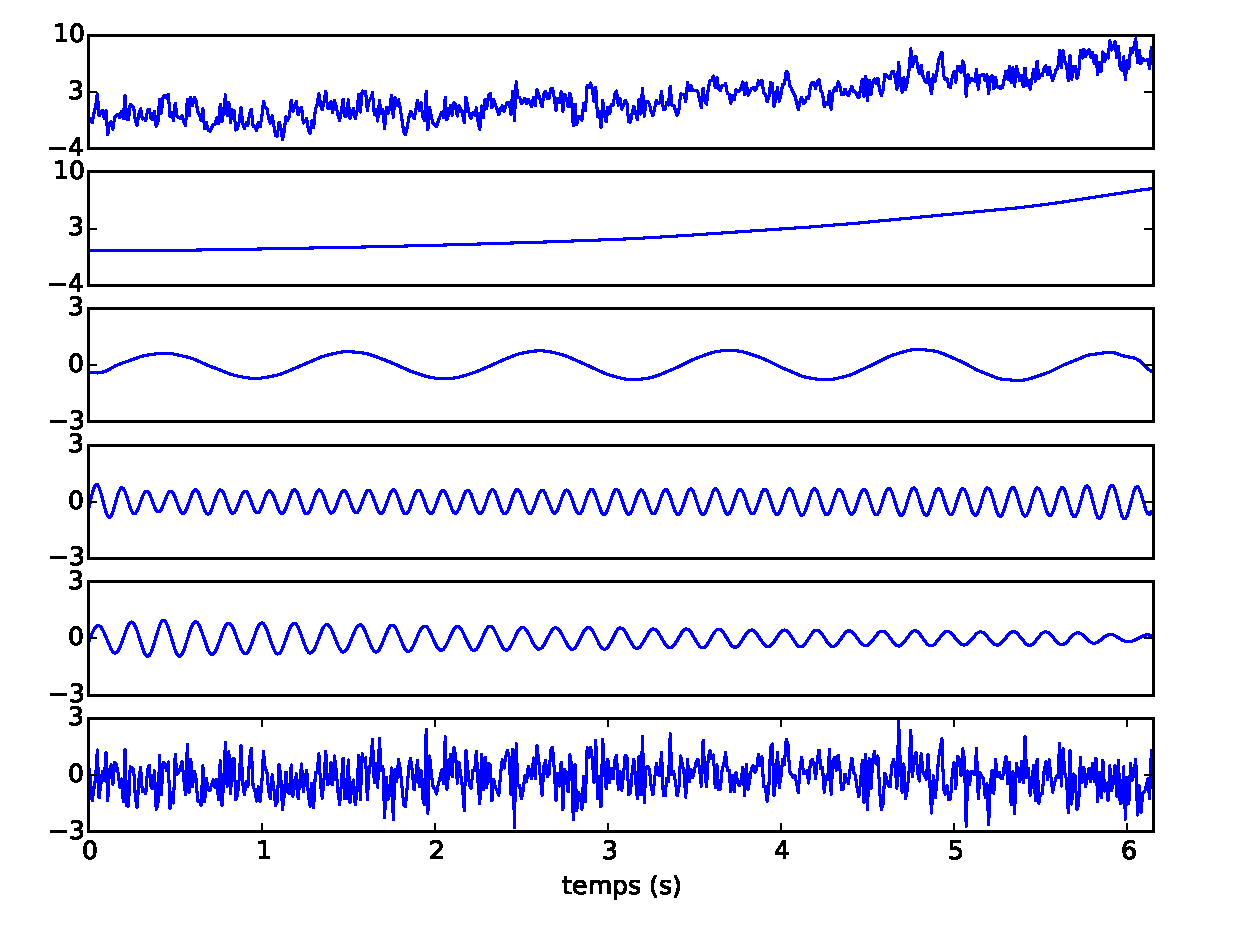
\includegraphics[width=.5\textwidth]{img/artsig3.eps}
        %\vspace{-.4cm}
        \caption{Décomposition d'un signal artificiel (\emph{haut}). Les quatres composantes du milieu correspondent aux groupes formés après la SSA par (HG)-(MH). Le signal du bas correspond au résiduel de la décomposition. On notera que les échelles des quatres signaux du bas ont été adaptées pour ne pas écraser les signaux.} %Le regroupement retrouve correctement plusieurs composantes harmoniques. Le bruits est largement filtré du signal de départ. Il n'est pas totalement gaussien car il intègre une composante harmonique du signal de départ qui n'est pas séparée par la décomposition du fait de sa trop faible amplitude.}
        \label{fig:dec}
    \end{figure}

%2/ Toutes les classes
%R_r 17.91%
%P_r 50.57%
%S_r 46.16%
Les méthodes ont été testées sur 100 signaux pour chacune des 3 classes, et les résultats moyennés sont reportés dans le Tableau \ref{tab:res}.
Pour la métrique $R_r$ calculées sur l'ensemble de la base de signaux tests (3 classes), l'utilisation de la méthode (HG)-(MH) donne un résultat statistiquement meilleur (au sens du test de Friedman) que les autres méthodes avec une amélioration moyenne de 48.4\%.
Pour $P_r$ et $S_r$, la méthode (KM) est statistiquement meilleure que les autres.
Elle permet d'obtenir une amélioration moyenne de $P_r$ de 80.4\% et de 63.9\% pour $S_r$.
L'estimation du nombre de composantes précise dans (KM) explique la précision largement meilleur que les autres ce qui se traduit aussi dans $S_r$.


%3/ Classes par classes
\begin{sloppypar}
Lorsqu'on les résultats uniquement sur la classe 1, on observe que (HG)-(MH) est statistiquement équivalente en rappel à (HGS)-(MU) et (HGS)-(MH). 
Pour les deux autres métriques, (HG)-(MH) et (HGS)-(MH) sont équivalentes et donnent un meilleur score que (KM).
Ces deux similarité sont particulièrement adaptées à la reconstruction d'harmonique pure ce qui explique leurs performances sur la classe 1. 
Pour les spectres très concentrés, elles donnent des résultats similaires ce qui explique leur proximité.
Pour les classes 2 et 3, (KM) est équivalente à (HGS)-(MH) pour $R_r$ et statistiquement meilleure que les autres méthodes pour les deux autres métriques.
%Lorsqu'on regarde les résultats classe par classe, on voit cependant que lorsque la complexité de la classe augmente, les différences sont de moins en moins significatives entre (HG)-(MH) et les autres méthodes.
%Pour $R_r$, (HG)-(MH) est statistiquement meilleure que (HGS)-(MU) pour les classes 1 et 2 mais pas pour la classe 3.
%Pour $P_r$, sur chaque classe séparément, cinq méthodes ont des performances comparables bien que (HG)-(MH) donne une meilleure performance moyenne et pour la classe 3, (HGS)-(MU) a une meilleure précision que (HG)-(MH).
%Ceci montre que si la méthode (HG)-(MH) semble la plus appropriée pour le groupement automatique pour des signaux composés d'harmoniques modulées, les autres méthodes peuvent donner des résultats intéressants pour des signaux avec des périodogrammes moins compacts.
%5/ Par composantes
Cette analyse est étayée par l'étude des résultats pour chaque type de composantes.
Le coefficient de détermination $r^2$ moyen obtenu pour la composante $c_0$ dans les classes 2 et 3 est en probabilité plus grand avec la méthode (KM) que pour les dix autres méthodes (cette méthode ne varie pas avec le choix de la stratégie de formation des groupes). 
Cette méthode observe l'intégralité du contenu fréquentiel pour effectuer le groupement ce qui est un avantage pour retrouver la composante de tendance qui peut avoir un périodogramme plus étalée. 
Pour les composantes harmoniques dans les classes 1 et 2, la méthode (HGS)-(MH) donne statistiquement un meilleur score $r^2$ sauf pour (HG)-(MH). 
Ces composantes sont particulièrement adaptées à la similarité basée sur leurs périodogrammes car ils ne sont composés que d'un pic.
Pour les composantes exponentiellement modulées, toutes les méthodes donnent des résultats statistiquement équivalents.
\end{sloppypar}

%4/ Méthode par méthode

\begin{table}[h]
\begin{tabular}{|c|c|c|c|c|c|c|}
	\hline
	Méthodes & GG1 & GG2 & GG3 & HG & KM & HGS\\\hline 
	$R_r$ - MU & 0.426 & 0.33 & 0.436 & 0.402 & 0.395 & 0.475\\\hline
$R_r$ - MH & 0.427 & 0.367 & 0.437 & \textbf{0.484} & 0.396 & 0.459\\\hline
$P_r$ - MU & 0.338 & 0.329 & 0.351 & 0.693 & 0.804 & 0.409\\\hline
$P_r$ - MH & 0.339 & 0.347 & 0.351 & 0.705 & \textbf{0.804} & 0.439\\\hline
$S_r$ - MU & 0.361 & 0.373 & 0.373 & 0.567 & 0.639 & 0.422\\\hline
$S_r$ - MH & 0.361 & 0.389 & 0.373 & 0.592 & \textbf{0.639} & 0.437\\\hline

\end{tabular}
\caption{\'Evaluation des différentes méthodes de groupement moyennée sur les 1000 signaux de chacune des classes de la base de test. Les 3 premières ligne présentent la stratégie de formation (MU) et les 3 suivantes la stratégie (MH).}
\label{tab:res}
\end{table}

\vspace{-.3cm}
\section{Conclusion}
\label{sec:ccl}

Le cadre général introduit pour la comparaison des stratégies de regroupement permet de voir que la méthode (HG)-(MH) est la plus adaptée à l'extraction de signaux harmoniques. Une étude plus poussé montre cependant que cette technique ne permet pas de retrouver aisément la tendance qui est plus facilement récupérer par (KM). Ces résultats prometteurs sont en cours d'adaptation pour l'étude de signaux physiologiques d'oculométrie.


\bibliographystyle{plain} 
\scriptsize
\bibliography{bib_dl2}{}
\end{document}
